% Options for packages loaded elsewhere
\PassOptionsToPackage{unicode}{hyperref}
\PassOptionsToPackage{hyphens}{url}
\PassOptionsToPackage{dvipsnames,svgnames,x11names}{xcolor}
%
\documentclass[
  letterpaper,
  DIV=11,
  numbers=noendperiod]{scrartcl}

\usepackage{amsmath,amssymb}
\usepackage{lmodern}
\usepackage{iftex}
\ifPDFTeX
  \usepackage[T1]{fontenc}
  \usepackage[utf8]{inputenc}
  \usepackage{textcomp} % provide euro and other symbols
\else % if luatex or xetex
  \usepackage{unicode-math}
  \defaultfontfeatures{Scale=MatchLowercase}
  \defaultfontfeatures[\rmfamily]{Ligatures=TeX,Scale=1}
\fi
% Use upquote if available, for straight quotes in verbatim environments
\IfFileExists{upquote.sty}{\usepackage{upquote}}{}
\IfFileExists{microtype.sty}{% use microtype if available
  \usepackage[]{microtype}
  \UseMicrotypeSet[protrusion]{basicmath} % disable protrusion for tt fonts
}{}
\makeatletter
\@ifundefined{KOMAClassName}{% if non-KOMA class
  \IfFileExists{parskip.sty}{%
    \usepackage{parskip}
  }{% else
    \setlength{\parindent}{0pt}
    \setlength{\parskip}{6pt plus 2pt minus 1pt}}
}{% if KOMA class
  \KOMAoptions{parskip=half}}
\makeatother
\usepackage{xcolor}
\setlength{\emergencystretch}{3em} % prevent overfull lines
\setcounter{secnumdepth}{-\maxdimen} % remove section numbering
% Make \paragraph and \subparagraph free-standing
\ifx\paragraph\undefined\else
  \let\oldparagraph\paragraph
  \renewcommand{\paragraph}[1]{\oldparagraph{#1}\mbox{}}
\fi
\ifx\subparagraph\undefined\else
  \let\oldsubparagraph\subparagraph
  \renewcommand{\subparagraph}[1]{\oldsubparagraph{#1}\mbox{}}
\fi

\usepackage{color}
\usepackage{fancyvrb}
\newcommand{\VerbBar}{|}
\newcommand{\VERB}{\Verb[commandchars=\\\{\}]}
\DefineVerbatimEnvironment{Highlighting}{Verbatim}{commandchars=\\\{\}}
% Add ',fontsize=\small' for more characters per line
\usepackage{framed}
\definecolor{shadecolor}{RGB}{241,243,245}
\newenvironment{Shaded}{\begin{snugshade}}{\end{snugshade}}
\newcommand{\AlertTok}[1]{\textcolor[rgb]{0.68,0.00,0.00}{#1}}
\newcommand{\AnnotationTok}[1]{\textcolor[rgb]{0.37,0.37,0.37}{#1}}
\newcommand{\AttributeTok}[1]{\textcolor[rgb]{0.40,0.45,0.13}{#1}}
\newcommand{\BaseNTok}[1]{\textcolor[rgb]{0.68,0.00,0.00}{#1}}
\newcommand{\BuiltInTok}[1]{\textcolor[rgb]{0.00,0.23,0.31}{#1}}
\newcommand{\CharTok}[1]{\textcolor[rgb]{0.13,0.47,0.30}{#1}}
\newcommand{\CommentTok}[1]{\textcolor[rgb]{0.37,0.37,0.37}{#1}}
\newcommand{\CommentVarTok}[1]{\textcolor[rgb]{0.37,0.37,0.37}{\textit{#1}}}
\newcommand{\ConstantTok}[1]{\textcolor[rgb]{0.56,0.35,0.01}{#1}}
\newcommand{\ControlFlowTok}[1]{\textcolor[rgb]{0.00,0.23,0.31}{#1}}
\newcommand{\DataTypeTok}[1]{\textcolor[rgb]{0.68,0.00,0.00}{#1}}
\newcommand{\DecValTok}[1]{\textcolor[rgb]{0.68,0.00,0.00}{#1}}
\newcommand{\DocumentationTok}[1]{\textcolor[rgb]{0.37,0.37,0.37}{\textit{#1}}}
\newcommand{\ErrorTok}[1]{\textcolor[rgb]{0.68,0.00,0.00}{#1}}
\newcommand{\ExtensionTok}[1]{\textcolor[rgb]{0.00,0.23,0.31}{#1}}
\newcommand{\FloatTok}[1]{\textcolor[rgb]{0.68,0.00,0.00}{#1}}
\newcommand{\FunctionTok}[1]{\textcolor[rgb]{0.28,0.35,0.67}{#1}}
\newcommand{\ImportTok}[1]{\textcolor[rgb]{0.00,0.46,0.62}{#1}}
\newcommand{\InformationTok}[1]{\textcolor[rgb]{0.37,0.37,0.37}{#1}}
\newcommand{\KeywordTok}[1]{\textcolor[rgb]{0.00,0.23,0.31}{#1}}
\newcommand{\NormalTok}[1]{\textcolor[rgb]{0.00,0.23,0.31}{#1}}
\newcommand{\OperatorTok}[1]{\textcolor[rgb]{0.37,0.37,0.37}{#1}}
\newcommand{\OtherTok}[1]{\textcolor[rgb]{0.00,0.23,0.31}{#1}}
\newcommand{\PreprocessorTok}[1]{\textcolor[rgb]{0.68,0.00,0.00}{#1}}
\newcommand{\RegionMarkerTok}[1]{\textcolor[rgb]{0.00,0.23,0.31}{#1}}
\newcommand{\SpecialCharTok}[1]{\textcolor[rgb]{0.37,0.37,0.37}{#1}}
\newcommand{\SpecialStringTok}[1]{\textcolor[rgb]{0.13,0.47,0.30}{#1}}
\newcommand{\StringTok}[1]{\textcolor[rgb]{0.13,0.47,0.30}{#1}}
\newcommand{\VariableTok}[1]{\textcolor[rgb]{0.07,0.07,0.07}{#1}}
\newcommand{\VerbatimStringTok}[1]{\textcolor[rgb]{0.13,0.47,0.30}{#1}}
\newcommand{\WarningTok}[1]{\textcolor[rgb]{0.37,0.37,0.37}{\textit{#1}}}

\providecommand{\tightlist}{%
  \setlength{\itemsep}{0pt}\setlength{\parskip}{0pt}}\usepackage{longtable,booktabs,array}
\usepackage{calc} % for calculating minipage widths
% Correct order of tables after \paragraph or \subparagraph
\usepackage{etoolbox}
\makeatletter
\patchcmd\longtable{\par}{\if@noskipsec\mbox{}\fi\par}{}{}
\makeatother
% Allow footnotes in longtable head/foot
\IfFileExists{footnotehyper.sty}{\usepackage{footnotehyper}}{\usepackage{footnote}}
\makesavenoteenv{longtable}
\usepackage{graphicx}
\makeatletter
\def\maxwidth{\ifdim\Gin@nat@width>\linewidth\linewidth\else\Gin@nat@width\fi}
\def\maxheight{\ifdim\Gin@nat@height>\textheight\textheight\else\Gin@nat@height\fi}
\makeatother
% Scale images if necessary, so that they will not overflow the page
% margins by default, and it is still possible to overwrite the defaults
% using explicit options in \includegraphics[width, height, ...]{}
\setkeys{Gin}{width=\maxwidth,height=\maxheight,keepaspectratio}
% Set default figure placement to htbp
\makeatletter
\def\fps@figure{htbp}
\makeatother

\KOMAoption{captions}{tableheading}
\makeatletter
\makeatother
\makeatletter
\makeatother
\makeatletter
\@ifpackageloaded{caption}{}{\usepackage{caption}}
\AtBeginDocument{%
\ifdefined\contentsname
  \renewcommand*\contentsname{Table of contents}
\else
  \newcommand\contentsname{Table of contents}
\fi
\ifdefined\listfigurename
  \renewcommand*\listfigurename{List of Figures}
\else
  \newcommand\listfigurename{List of Figures}
\fi
\ifdefined\listtablename
  \renewcommand*\listtablename{List of Tables}
\else
  \newcommand\listtablename{List of Tables}
\fi
\ifdefined\figurename
  \renewcommand*\figurename{Figure}
\else
  \newcommand\figurename{Figure}
\fi
\ifdefined\tablename
  \renewcommand*\tablename{Table}
\else
  \newcommand\tablename{Table}
\fi
}
\@ifpackageloaded{float}{}{\usepackage{float}}
\floatstyle{ruled}
\@ifundefined{c@chapter}{\newfloat{codelisting}{h}{lop}}{\newfloat{codelisting}{h}{lop}[chapter]}
\floatname{codelisting}{Listing}
\newcommand*\listoflistings{\listof{codelisting}{List of Listings}}
\makeatother
\makeatletter
\@ifpackageloaded{caption}{}{\usepackage{caption}}
\@ifpackageloaded{subcaption}{}{\usepackage{subcaption}}
\makeatother
\makeatletter
\@ifpackageloaded{tcolorbox}{}{\usepackage[many]{tcolorbox}}
\makeatother
\makeatletter
\@ifundefined{shadecolor}{\definecolor{shadecolor}{rgb}{.97, .97, .97}}
\makeatother
\makeatletter
\makeatother
\ifLuaTeX
  \usepackage{selnolig}  % disable illegal ligatures
\fi
\IfFileExists{bookmark.sty}{\usepackage{bookmark}}{\usepackage{hyperref}}
\IfFileExists{xurl.sty}{\usepackage{xurl}}{} % add URL line breaks if available
\urlstyle{same} % disable monospaced font for URLs
\hypersetup{
  pdftitle={PPO for humans},
  colorlinks=true,
  linkcolor={blue},
  filecolor={Maroon},
  citecolor={Blue},
  urlcolor={Blue},
  pdfcreator={LaTeX via pandoc}}

\title{PPO for humans}
\author{}
\date{2023-11-08}

\begin{document}
\maketitle
\ifdefined\Shaded\renewenvironment{Shaded}{\begin{tcolorbox}[sharp corners, enhanced, boxrule=0pt, borderline west={3pt}{0pt}{shadecolor}, frame hidden, breakable, interior hidden]}{\end{tcolorbox}}\fi

\renewcommand*\contentsname{Table of contents}
{
\hypersetup{linkcolor=}
\setcounter{tocdepth}{3}
\tableofcontents
}
\hypertarget{neural-networks}{%
\subsection{Neural networks}\label{neural-networks}}

For PPO, we have two neural networks:

\begin{itemize}
\tightlist
\item
  the action network \texttt{action\_net}
\item
  the value network \texttt{value\_net}
\end{itemize}

\begin{figure}

{\centering 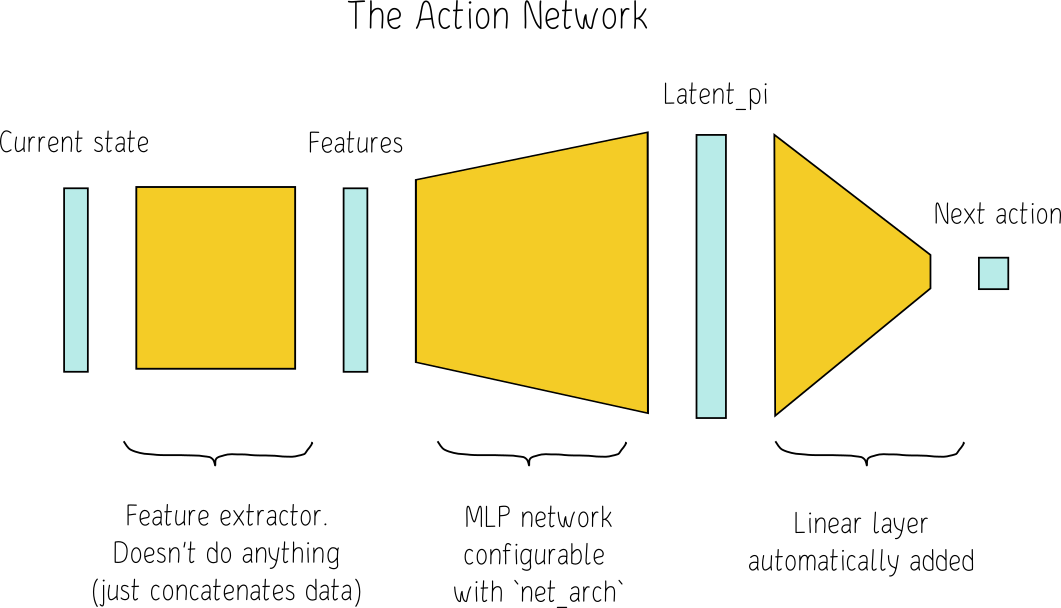
\includegraphics{img/ActionNet.png}

}

\caption{Overview of the Action Net}

\end{figure}

\hfill\break

\begin{figure}

{\centering 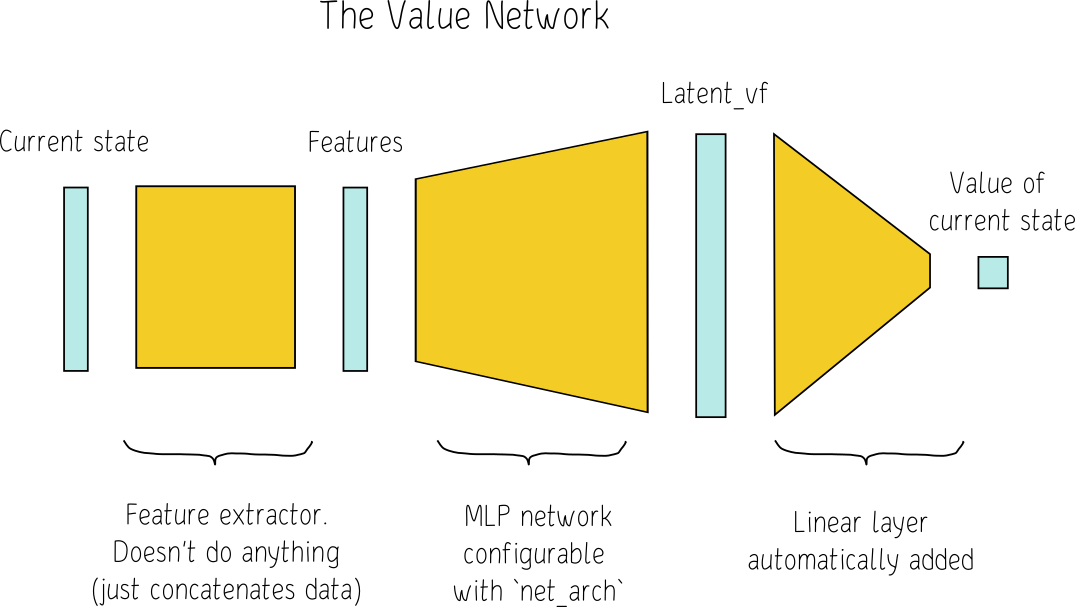
\includegraphics{img/ValueNet.png}

}

\caption{Overview of the Value Net}

\end{figure}

Both networks are joined together in a single PyTorch network object,
whose \texttt{forward()} function (the forward pass) is the following
(from
\texttt{/data/venv/cnc-rl/lib/python3.11/site-packages/stable\_baselines3/common/policies.py}):

\begin{Shaded}
\begin{Highlighting}[]
\KeywordTok{def}\NormalTok{ forward(}\VariableTok{self}\NormalTok{, obs: th.Tensor, deterministic: }\BuiltInTok{bool} \OperatorTok{=} \VariableTok{False}\NormalTok{) }\OperatorTok{{-}\textgreater{}}\NormalTok{ Tuple[th.Tensor, th.Tensor, th.Tensor]:}
    \CommentTok{"""}
\CommentTok{    Forward pass in all the networks (actor and critic)}

\CommentTok{    :param obs: Observation}
\CommentTok{    :param deterministic: Whether to sample or use deterministic actions}
\CommentTok{    :return: action, value and log probability of the action}
\CommentTok{    """}
    \CommentTok{\# Preprocess the observation if needed}
\NormalTok{    features }\OperatorTok{=} \VariableTok{self}\NormalTok{.extract\_features(obs)}
    \ControlFlowTok{if} \VariableTok{self}\NormalTok{.share\_features\_extractor:}
\NormalTok{        latent\_pi, latent\_vf }\OperatorTok{=} \VariableTok{self}\NormalTok{.mlp\_extractor(features)}
    \ControlFlowTok{else}\NormalTok{:}
\NormalTok{        pi\_features, vf\_features }\OperatorTok{=}\NormalTok{ features}
\NormalTok{        latent\_pi }\OperatorTok{=} \VariableTok{self}\NormalTok{.mlp\_extractor.forward\_actor(pi\_features)}
\NormalTok{        latent\_vf }\OperatorTok{=} \VariableTok{self}\NormalTok{.mlp\_extractor.forward\_critic(vf\_features)}
    \CommentTok{\# Evaluate the values for the given observations}
\NormalTok{    values }\OperatorTok{=} \VariableTok{self}\NormalTok{.value\_net(latent\_vf)}
\NormalTok{    distribution }\OperatorTok{=} \VariableTok{self}\NormalTok{.\_get\_action\_dist\_from\_latent(latent\_pi)}
\NormalTok{    actions }\OperatorTok{=}\NormalTok{ distribution.get\_actions(deterministic}\OperatorTok{=}\NormalTok{deterministic)}
\NormalTok{    log\_prob }\OperatorTok{=}\NormalTok{ distribution.log\_prob(actions)}
\NormalTok{    actions }\OperatorTok{=}\NormalTok{ actions.reshape((}\OperatorTok{{-}}\DecValTok{1}\NormalTok{, }\OperatorTok{*}\VariableTok{self}\NormalTok{.action\_space.shape))}
    \ControlFlowTok{return}\NormalTok{ actions, values, log\_prob}
\end{Highlighting}
\end{Shaded}

\hypertarget{ppo-training}{%
\subsection{PPO training}\label{ppo-training}}

The main loop in PPO consists of two steps:

\begin{enumerate}
\def\labelenumi{\arabic{enumi}.}
\tightlist
\item
  Repeat

  \begin{enumerate}
  \def\labelenumii{\arabic{enumii}.}
  \tightlist
  \item
    Rollout

    \begin{itemize}
    \tightlist
    \item
      play simulations with current policy (i.e.~current Action Net) and
      collect rewards
    \item
      doesn't update anything
    \item
      it's here where distribution sampling is done, during simulations
    \end{itemize}
  \item
    Train

    \begin{itemize}
    \tightlist
    \item
      train neural networks according to PPO learning algorithm, using
      the data recorded during the rollout stage
    \item
      distribution is not sampled here, but it needs to recompute the
      probability of the actions recorded during collection
    \end{itemize}
  \end{enumerate}
\end{enumerate}

The general idea of PPO training is:

\begin{enumerate}
\def\labelenumi{\arabic{enumi}.}
\tightlist
\item
  During rollout, collect the cumulative reward (i.e.~value) out of
  every state, to act like a ground truth

  \begin{itemize}
  \tightlist
  \item
    This uses the current policy, i.e.~current Action Net, when sampling
    actions
  \item
    Record all the tuples
    \texttt{(state,\ action\ taken,\ cumulative\ reward)}
  \end{itemize}
\item
  Compute the estimated value of the same states with the Value Net
\item
  Compare and update:

  \begin{itemize}
  \tightlist
  \item
    look back on all the
    \texttt{(state,\ action\ taken,\ cumulative\ reward)} tuples
    collected, and:
  \item
    for actions leading to states where the Value Net output is larger
    than observed ground truth value, decrease the probability of those
    actions (i.e.~we overestimated those actions' worth, compared to
    ground truth)
  \item
    for actions leading to states where the Value Net output is smaller
    than observed ground truth value, increase the probability of those
    actions (i.e.~we underestimated those action' worth, compared to
    ground truth)
  \end{itemize}
\end{enumerate}

The equilibrium state, when both Action Net and Value Net are fully
converged, is when the cumulative rewards collected in the rollout
stage, with the current Action Net (current policy), are identical to
those states' values as computed by the Value Net.

\hypertarget{sampling-mechanism}{%
\subsection{Sampling mechanism}\label{sampling-mechanism}}

Sampling depends on how the policy (action probability distribution) is
parameterized.

The underlying distributions are the ones from PyTorch (see below, from
\texttt{/data/venv/cnc-rl/lib/python3.11/site-packages/stable\_baselines3/common/policies.py}):

\begin{Shaded}
\begin{Highlighting}[]
\ImportTok{from}\NormalTok{ torch.distributions }\ImportTok{import}\NormalTok{ Bernoulli, Categorical, Normal}
\end{Highlighting}
\end{Shaded}

\begin{Shaded}
\begin{Highlighting}[]
  \KeywordTok{def}\NormalTok{ \_get\_action\_dist\_from\_latent(}\VariableTok{self}\NormalTok{, latent\_pi: th.Tensor) }\OperatorTok{{-}\textgreater{}}\NormalTok{ Distribution:}
      \CommentTok{"""}
\CommentTok{      Retrieve action distribution given the latent codes.}

\CommentTok{      :param latent\_pi: Latent code for the actor}
\CommentTok{      :return: Action distribution}
\CommentTok{      """}
\NormalTok{      mean\_actions }\OperatorTok{=} \VariableTok{self}\NormalTok{.action\_net(latent\_pi)}

      \ControlFlowTok{if} \BuiltInTok{isinstance}\NormalTok{(}\VariableTok{self}\NormalTok{.action\_dist, DiagGaussianDistribution):}
          \ControlFlowTok{return} \VariableTok{self}\NormalTok{.action\_dist.proba\_distribution(mean\_actions, }\VariableTok{self}\NormalTok{.log\_std)}
      \ControlFlowTok{elif} \BuiltInTok{isinstance}\NormalTok{(}\VariableTok{self}\NormalTok{.action\_dist, CategoricalDistribution):}
          \CommentTok{\# Here mean\_actions are the logits before the softmax}
          \ControlFlowTok{return} \VariableTok{self}\NormalTok{.action\_dist.proba\_distribution(action\_logits}\OperatorTok{=}\NormalTok{mean\_actions)}
      \ControlFlowTok{elif} \BuiltInTok{isinstance}\NormalTok{(}\VariableTok{self}\NormalTok{.action\_dist, MultiCategoricalDistribution):}
          \CommentTok{\# Here mean\_actions are the flattened logits}
          \ControlFlowTok{return} \VariableTok{self}\NormalTok{.action\_dist.proba\_distribution(action\_logits}\OperatorTok{=}\NormalTok{mean\_actions)}
      \ControlFlowTok{elif} \BuiltInTok{isinstance}\NormalTok{(}\VariableTok{self}\NormalTok{.action\_dist, BernoulliDistribution):}
          \CommentTok{\# Here mean\_actions are the logits (before rounding to get the binary actions)}
          \ControlFlowTok{return} \VariableTok{self}\NormalTok{.action\_dist.proba\_distribution(action\_logits}\OperatorTok{=}\NormalTok{mean\_actions)}
      \ControlFlowTok{elif} \BuiltInTok{isinstance}\NormalTok{(}\VariableTok{self}\NormalTok{.action\_dist, StateDependentNoiseDistribution):}
          \ControlFlowTok{return} \VariableTok{self}\NormalTok{.action\_dist.proba\_distribution(mean\_actions, }\VariableTok{self}\NormalTok{.log\_std, latent\_pi)}
      \ControlFlowTok{else}\NormalTok{:}
          \ControlFlowTok{raise} \PreprocessorTok{ValueError}\NormalTok{(}\StringTok{"Invalid action distribution"}\NormalTok{)}
\end{Highlighting}
\end{Shaded}

\hypertarget{continuous-actions}{%
\subsubsection{Continuous actions}\label{continuous-actions}}

For continuous actions, the distribution is parameterized a diagonal
gaussian:

\begin{itemize}
\tightlist
\item
  the mean is the value produced by the Action Net (size = action size)
\item
  the deviation is a separate learnable parameter (size = 1, same value
  for all dimensions)
\end{itemize}

Sampling is done using the same reparameterization trick as in
Variational Autoencoders: sample the standard normal, then multiply with
deviation and add mean.

During evaluation runs, when we want the most likely action and not a
sample, we simply take the output of the Action Net, i.e.~the mean
action.

During our simulation, choosing the next step is therefore choosing a
point from a gaussian cloud:

\hfill\break

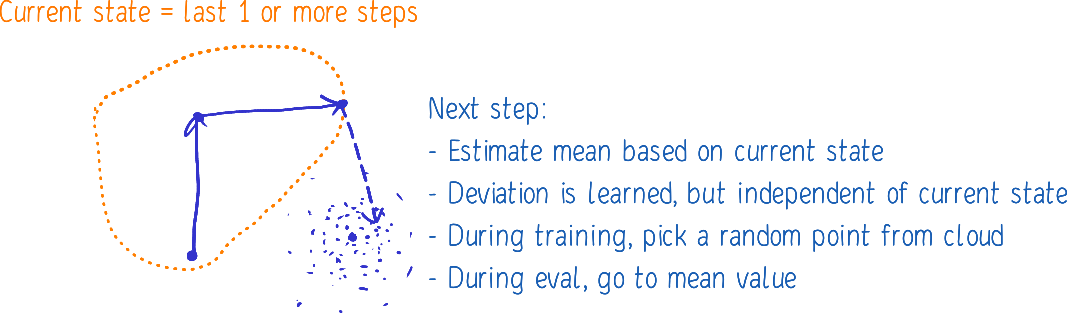
\includegraphics{img/Explanation.png}

\hypertarget{discrete-actions}{%
\subsubsection{Discrete actions}\label{discrete-actions}}

For discrete actions, the distribution is a categorical distribution

\begin{itemize}
\tightlist
\item
  Action Net produces directly the probabilities (or logits) of every
  action (vector size = action size)
\item
  sampling is done with PyTorch.
\end{itemize}



\end{document}
